\clearpage\begingroup\SourceLeaf{41b}\HistoricalHead{36}{L}{PHYSIK. BRIEFWECHSEL.}
\begin{center}
[4.]\\[.7em]
\textsc{Gauss} an \textsc{Gerling}. Göttingen, 28. Februar 1852.
\end{center}
\noindent .\ .\ .\ .\ .\ .\ .\ .\ .\ .\ .\ .\ .\ .\ .\ .\ .\ .\ .\ .\ .
\par\noindent\hspace*{\parindent}Die mathematische Behandlung der Pendelschwingungen auf der rotirenden
Erde ist, wie Sie aus den A. N. wissen werden, von der Danziger Naturf. Gesellschaft
zum Gegenstande einer Preisfrage gemacht[\textsuperscript{*})]\begingroup\renewcommand{\thefootnote}{}\footnotetext{[\textsuperscript{*}) Die in den Astronomischen Nachrichten \textbf{34}, 1852, Spalte 33 veröffentlichte und vom 4. Februar 1852 datierte Preisaufgabe lautete: »Die Bewegung des Pendels mit \textls[120]{Rücksicht auf die Umdrehung der Erde}, im Sinne \textsc{Lagranges}, nämlich etwa so zu behandeln, wie der große Analytiker sie würde durchgeführt haben, wenn er sie zum Gegenstande seiner Untersuchung gemacht hätte«. Die Einsendungsfrist endete am 1. Oktober 1852.]}\endgroup. Mir will das Programm
nicht recht gefallen. Erstlich ist die Frist zu kurz. Nicht jeder, der etwa
befähigt wäre, ist in solchem Maasse Herr seiner Zeit, um eine in keiner
Weise mechanische Arbeit so schnell zu vollenden, dass sie schon vor Ende
September d. J. eingesandt sein kann. Dann sieht man nicht bestimmt genug,
wieviel eigentlich gefordert wird. Wenn nur eine Behandlung, wie die \textsc{Lagrange}sche,
bloss unter Zusatz der Wirkungen der Erdrotation gefordert wird,
so lässt schon die \textsc{Plana}sche Arbeit nichts zu wünschen übrig, und enthält
so feine Mathematik, dass es leicht möglich wäre, dass ein gekrönter Bewerber,
der erst hinterher die \textsc{Plana}sche Arbeit kennen lernte, nur den
bittersten Aerger fühlte. Die \textsc{Plana}sche Abhandlung ist im 13. Bande der
\clearpage\SourceLeaf{42}\HistoricalHead{37}{R}{GAUSS AN GERLING.}
\noindent Turiner Denkschriften 2. Serie enthalten[\textsuperscript{*})]\begingroup\renewcommand{\thefootnote}{}\footnotetext{[\textsuperscript{*}) J. \textsc{Plana}, \textit{Note sur l'expérience communiquée par Mr. L. Foucault le 3. février 1851 à l'Académie de Paris}, Memorie dell'Accademia delle Scienze di Torino, 2. ser. \textbf{13}, 1853.]}\endgroup. Ich habe \textsc{Weber} gebeten,
\textsc{Poggendorff} zu einer möglichst baldigen Uebersetzung für seine Annalen zu
veranlassen.

In Beziehung auf die Anstellung der Versuche habe ich auf eine andere
Methode gedacht, wobei das Reflexionsprincip benutzt werden kann. Ich bin
aber nach genauerer Ueberlegung davon zurückgekommen, das Pendel mit
einer konischen Spitze auf einer harten Fläche \(S\) aufsitzen zu lassen.

\noindent\begin{minipage}[t]{.74\textwidth}\vspace{0pt}\setlength{\parindent}{1.2em}\hspace*{\parindent}Ich denke mir, das Pendel hängt an einem eingeklemmten
Draht, der aber nur etwa 1 Zoll lang und an
seinem untern Ende in eine steife Stange encastrirt ist.
Diese Stange, von mässiger Stärke und Länge, trägt unten
das Gewicht, eine Kugel oder vielleicht noch besser eine
Linse mit horizontalem Aequator. Oben an der Stange ist
ein Planspiegel, dessen Ebene im Augenblick des freien Herabhängens
des Pendels vertical ist, und um die Ideen zu
fixiren im Meridian gedacht werden mag, die reflektirende
Fläche nach Ost gerichtet. Als eine Verbesserung würde
ich noch ansehen, den Spiegel nicht unmittelbar an der
\end{minipage}\hfill\begin{minipage}[t]{.23\textwidth}\vspace{0pt}\centering
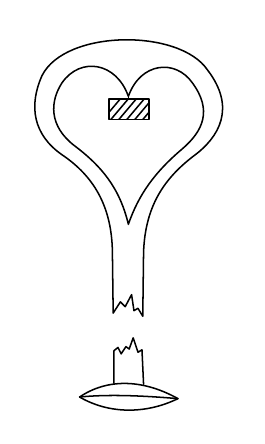
\begin{tikzpicture}[x=.004in,y=-.004in,line width=.55pt,line cap=round,line join=round]
\draw (113,353)--(112,276)
 .. controls (111,213) and (83,178) .. (49,155)
 .. controls (13,130) and (7,94) .. (24,56)
 .. controls (53,-2) and (196,-3) .. (231,49)
 .. controls (267,96) and (246,133) .. (213,157)
 .. controls (178,184) and (153,218) .. (151,277)
 --(150,357)--(144,347)--(139,350)--(136,330)--(128,345)--(122,339)--cycle;
\draw (132,242)
 .. controls (121,196) and (98,169) .. (65,144)
 .. controls (32,119) and (34,88) .. (49,65)
 .. controls (72,32) and (117,39) .. (132,82)
 .. controls (147,39) and (191,35) .. (212,65)
 .. controls (237,99) and (226,125) .. (199,148)
 .. controls (166,176) and (145,204) .. (132,242);
\draw (132,82)--(132,85);
\draw (108,85) rectangle (158,111);
\begin{scope}\clip (108,85) rectangle (158,111);
\foreach \x in {100,110,120,130,140,150,160}{\draw (\x,111)--(\x+22,85);}
\end{scope}
\draw (114,441)--(114,400)--(119,396)--(123,404)--(129,395)--(133,398)--(138,384)--(144,402)--(149,399)--(151,442);
\draw (71,458) .. controls (105,435) and (149,435) .. (194,460)
 .. controls (153,480) and (107,479) .. (71,458);
\draw (71,458) .. controls (111,454) and (158,457) .. (194,460);
\end{tikzpicture}\end{minipage}
\par\noindent Stange anzubringen, sondern an einem Arme, so dass die Mitte des Spiegels
mit dem Aufhängungspunkte in Einer Höhe ist. Im Osten in schicklicher
Entfernung ist ein gegen den Spiegel gerichtetes Fernrohr, worin man das
Bild einer \textls[120]{verticalen} Scale sieht.

Versetzt man nun das Pendel in Schwingungen, und zwar so, dass die
Schwingungsebene der Meridian[ebene] (allgemein der Spiegelebene) parallel
ist, so dreht letztere sich nur in sich selbst um und das Scalenbild bleibt völlig
ruhig. Hat aber nach einiger Zeit das Azimuth der Schwingungsebene sich
geändert (von SW nach NO), so steigt das Scalenbild im Fernrohr auf und
nieder, oder was dasselbe ist, das Fadenkreuz scheint sich auf der Scala auf
und nieder zu bewegen.

\textsc{Weber} hat einen, allerdings nur erst sehr rohen Versuch der Ausführung
gemacht. Ich habe aber seine Einrichtung noch nicht selbst gesehen. Denn
meine Mobilität zu Fuss erstreckt sich seit \(\tfrac{1}{2}\) Jahre nicht weiter als von der
\clearpage\SourceLeaf{43}\HistoricalHead{38}{L}{PHYSIK. BRIEFWECHSEL.}
\noindent Sternwarte zum Museum und zurück. Nur Einmahl bin ich bis zum Universitätshause
gegangen, wobei ich meinen Athem ganz verlor. Inzwischen, nach dem
was er mir berichtet, werden bei einer solchen Einrichtung, wenn sie mit
aller Sorgfalt in angemessenen Dimensionen und Localität ausgeführt wird,
die Versuche eine Eleganz erhalten, wovon andere Einrichtungen weit entfernt
bleiben müssen. Schon bei \textsc{Webers} roher Einrichtung, Fernrohr in kleiner
Entfernung, nicht fester, oft durch fahrende Wagen gestörter Aufstellung, betrug
die Amplitude der Bildbewegung schon nach \textls[120]{einer Minute} etwa
3 Scalentheile oder Millimeter. Es versteht sich, dass wenn die ursprüngliche
Bewegung in einem etwas kleinern Azimuth (SO nach NW) geschieht,
gleich Anfangs eine auf- und abgehende Bildbewegung vorhanden ist, die nach
und nach schwächer wird, bis sie in die entgegengesetzte übergeht. Ich
zweifle nicht, dass auf diese Art es möglich sein wird, die Erdrotation schon
nach wenigen Secunden erkennbar zu machen.\quad .\ .\ .\ .\ .\ .\ .\ .\ .\ .\ .\ .\ .\ .\ .\ .\ .
\clearpage\endgroup
